\documentclass{article}
\usepackage{graphicx}
\usepackage{tikz}
\usepackage{pgfplots}
\usepackage[margin=2.5cm]{geometry}
\usepackage{amssymb}
\usepackage{biblatex}
\usepackage{booktabs}
\usepackage{array}
\usepackage{amsmath}
\usepackage{listings}
\lstset{basicstyle=\ttfamily,
	showstringspaces=false,
	commentstyle=\color{red},
	keywordstyle=\color{blue}
}

\usepackage{pgfplots}
\usepackage[colorlinks=true,allcolors=black]{hyperref}
%\usepackage[backend=biber, bibencoding=utf8, style=ieee]{biblatex}

\addbibresource{references.bib}

\begin{document}
\title{ {\fontsize{16}{1} \selectfont Control over an embedded computing platform} {\\ \fontsize{13}{1} \selectfont \textbf{Embedded Control Systems}} }
\author{Sai Krishna Kalluri \& Snorri Stefansson }

\maketitle
%
%Modified	CompSOC configuration	file	(sconfig.c)
%• System	states	and	control	input	traces	from	the	CompSOC platform	(states.txt,	
%input.txt)
%• Makefile used	to	specify	the	USER_TIMEOUT	(makefile)
%• MATLAB	control	design	script	(stud_control_design_a1.m)
%• A	report	of	no	more	than	10	pages	describing	(a1.pdf

%• Report	should	be	written	in	English
\section{Introduction}
%Brief	introduction	of	the	overall	setting
The goal of this project is to design control parameters for motor-mass-spring fourth order SIMO (Singlu Input Multiple Output) system. First of all it is important to understand the physical components of the system and which sensor and actuator are present.

A input signal (current, A) is applied to a motor(object 1) which will turn a spring which is connected to a mass which rotates (object 2). Both objects have encoders and are used to close the loop of the control system, acting as feedback. A few more values are affect the systems like inertia (shape), torque, value of mass, spring characteristic and friction.

This assignment is not only designing control parameters but also interfering with a simulator for the plant. The simulator acts not as a continuous systems but a discrete system with sampling period of 100 $\mu$s. This has to be taken into account during the design in order to. The simulator is a FPGA running xlinux like many high-end FPGAs. 





\section{System Model Derivation and Control Parameter Design}
%System	model	derivation	and	controller	parameter	design
The objectives for the controller is to properly control the given system with a set of design parameters. These parameters, shown in Table \ref{tab:design}, have to be design and put into perspective with our system, which role they play and the best way to derive them adequately.

There are namely a number of steps taken until all parameters can be considered to satisfy the performance constraints of the controller. These basic steps can be seen in the following list.

\begin{enumerate}
	\item Step 1: Derive the system model. Determine the A, B and C matrices in relation to all constants by hand calculations. Inserting this into Matlab. These calculations can be seen in Section \ref{sec:controllerstructure} in full detail.
	\item Step 2: Forming sensible values for C,P TDM\_TABLE\_Size and DELAY. The relationship between these values was inspected in full detail and is discussed in Section \ref{sec:platform}
	\item Step 3: Determine the locations of Ts, Tc and Ta in the TDM table.
	\item Step 4: Determining the sensor to actuator delay in relation to the chosen design parameters, especially P, C and TDM table size is calculated and discussed in Section \ref{sec:stad}. 
	\item Step 5: Simulation for all determined parameters is run and checked if they meet all performance constraints. The check on the performance constraints is also performed during Step 2 by running a script for all parameters and checking every time. This is discussed in more detail in Section \ref{sec:platform}.
	\item Step 6: Finally modifying the Sconfig.c file in the platform to match the design parameters.\color{red} ADD REFERENCE TO SECTION WHEN FINIHSED WRITING ABOUT IT ;) \color{black}
	\item Step 7: Generate both actuator and sensor output files from the platform to feed to Matlab to compare the results with ones from Simulink.\color{red} ADD REFERENCE TO SECTION WHEN FINIHSED WRITING ABOUT IT ;) \color{black}
\end{enumerate}


\begin{table}[h!]
	\centering
	\caption{Design parameters and deliverables for the model. The poles are also something that has to be design or chosen but that will be discussed in Section \ref{sec:controllerstructure}}
	\begin{tabular}{lll}
		\toprule
		Design Parameter & Symbol/Referenced as &Unit\\
		\midrule
		CoMik microkernel slot size& C & Clock Cycles \\
		Partition slot size& P & Clock Cycles\\
		TDM table size& TDM\_TABLE\_SIZE & Natural Number larger than 2\\
		Partition slots allocation	& for Ts, Tc, and Ta & Location in TDM table \\
		Sensor-to-actuator	delay& DELAY & Clock Cycles	\\
		Feedback gain& K & 4x4 matrix \\
		Feedforward gain& F & 4x1 matrix \\
		\midrule		
	\end{tabular}
	\label{tab:design}
\end{table}

\begin{table}[htbp]
	\centering
	\caption{Constants referenced to in calculations}
	\begin{tabular}{llll}
		\toprule
		Symbol & Description & Value & Unit\\ 
		\midrule
		$\theta$ & Masses position  & -&rad \\ 
		$i_m$ & Motor current  & - &A \\ 
		J$_1 = J_2$ & Inertia  & $3.75\cdot10^{-6}$&$Kgm^2$  \\ 
		b & Friction  coefficient   &$ 1\cdot10^{-5} $&Nms/rad\\ 
		k & Torsional spring  & 0.2656 &Nm/rad\\
		d & Torsional damping  & $3.125\cdot10^{-5}$&Nms/rad \\ 
		$K_m$ & Motor constant  & $4.4\cdot10^{-2}$&Nm/A  \\ 
		\midrule
	\end{tabular}
	\label{}
\end{table}

 

\subsection{Controller Structure}
 \label{sec:controllerstructure}
The system can be described with the fourth order differential equation shown in Equation \ref{eq:1} and \ref{eq:2} which will be solved considering Equation \ref{eq:3}. From these equations the Feedback- and Feedforward gain can be determined in relations to the constants in the system.
%\color{red}
%Show some equations 
%\color{black}

\begin{equation}
J_1 \; \ddot{\theta}_1 = K_m \; i_m - k(\theta_1-\theta_2) - d(\dot{\theta}_1-\dot{\theta}_2) - b(\dot{\theta}_1-\dot{\theta}_2)
\label{eq:1}
\end{equation}

\begin{equation}
J_2 \; \ddot{\theta}_2 = -k(\theta_2-\theta_1) - d(\dot{\theta}_2-\dot{\theta}_1) - b(\dot{\theta}_2-\dot{\theta}_1)
\label{eq:2}
\end{equation}

\begin{equation}
\label{eq:3}
\text{\textit{\textbf{x}}}=
\begin{bmatrix}
x_1\\
x_2 \\
x_3 \\
x_4 
\end{bmatrix}
=
\begin{bmatrix}
\theta_1\\
 \theta_2\\
\dot{\theta_1}\\
\dot{\theta_2}
\end{bmatrix}
=
\begin{bmatrix}
\theta_1\\
\theta_2\\
\omega_1\\
\ \omega_2
\end{bmatrix}
\end{equation}

\begin{equation}
\dot{\text{\textit{\textbf{x}}}}(t) = \bar{\text{\textbf{A}}}\text{\textit{\textbf{x}}}(t) +  \bar{\text{\textbf{B}}}\text{\textit{\textbf{u}}}(t) \text{ and } \text{\textit{\textbf{y}}}(t) = \bar{\text{\textbf{C}}}\text{\textit{\textbf{x}}}(t) \qquad \text{ where } \quad \text{\textit{\textbf{u}}}=i_m \text{ and \textit{\textbf{y}}}=\theta_1
\end{equation}

\begin{equation}
\dot{\text{\textit{\textbf{x}}}} = \begin{bmatrix}
& & & \\[0.3em]
\text{\color{white}H\color{black}} &\text{\color{white}h\color{black}} &\text{\color{white}hh\color{black}} &\text{\color{white}hh\color{black}} \\
\text{\color{white}hh\color{black}}& & & \\
\text{\color{white}hh\color{black}} & & &
\end{bmatrix}
\begin{bmatrix}
\theta_1\\
\theta_2\\
\omega_1\\
\omega_2\\
\end{bmatrix}
+
\begin{bmatrix}
\text{\color{white}hh\color{black}}\\
\text{\color{white}hh\color{black}}\\
\text{\color{white}hh\color{black}}\\
\text{\color{white}hh\color{black}}\\
\end{bmatrix}\text{\textit{\textbf{u}}}
\quad \text{ and } \quad
\text{\textit{\textbf{y}}}=\begin{bmatrix}
\text{\color{white}hh\color{black}} &\text{\color{white}hh\color{black}}&\text{\color{white}hh\color{black}}&\text{\color{white}hh\color{black}}
\end{bmatrix}
\begin{bmatrix}
\theta_1\\
\theta_2\\
\omega_1\\
\omega_2\\
\end{bmatrix}
\label{eq:4}
\end{equation}
\section{Platform Parameter Design}
\label{sec:platform}

The microkernel slot size C, partition table size P and TDM table size in the control system design play a large role in task timing and scheduling. These parameters' units are shown in Table \ref{tab:design}. The mircokernel slot size will determine the the clock cycles (time) for which the microkernel needs to execute correctly, this was stated to be at least 40.96$\mu$s.

Thus the microkernel slot size could at best reach roughly 40 $\mu$s which would yield to about: $$ C_{min} = 100MHz \cdot 40.96 \mu s = 4096 \;\;Clock \; Cycles$$

This observation was small starting point of educated assumptions about which C and P to chose. Then it was decided rather than picking values for P and C separately to pick a fraction, relating those two. 

In Section \ref{sec:steps} the steps to the findings of sufficient values for P, C and TDM tabel size will be carried out. The goal is to meet the design constraints and at the same time have a good Quality of Control.
\subsection{Controller Design}
In this subsection we discuss the method for designing the controller design parameters FeedbackGain-$K$ and FeedForwardGain-$F$. In this problem we have the scenario where $D_c<h$. Since we our controller operates in discrete domain, we start with converting our continuous system into discrete domain. Therefore on applying ZOH sampling with period $h_c$ and constant sensor-actuator Delay $D_c$ we achieve the equation \ref{eq:code1}. From \ref{eq:code1} we can notice that the next output not only depends on current input but also n previous input. Hence, we simplify the system into equation \ref{eq:code2} after invoking .
Thus matrices $\Phi$ ,$C$ are converted to $\Phi_{aug}$,$C_{aug}$ whereas $\Gamma_1$,$\Gamma_2$ are converted to $\Gamma_{aug}$.

  Before deriving the controller gains it is important to verify if the system is controllable under given configuration. This can be verified by calculating $det(\gamma_{aug})$. If the determinent is not equal to 0, then system is controllable. After verifying the controllability of the system $K$ can be derived by applying Ackermanns formula \ref{eq:delay} and $F$ can be derived from eqaution .

\subsection{Design and Workflow}
\label{sec:steps}
This subsection will discuss selection of P,C, Sensor to actuator delay and some choices considered for poles, TDM table size in order to meet the design constraints. To create an overview of how this was done, a timeline with the steps taken will be presented here.

\begin{figure}[h!]
	\begin{center}
		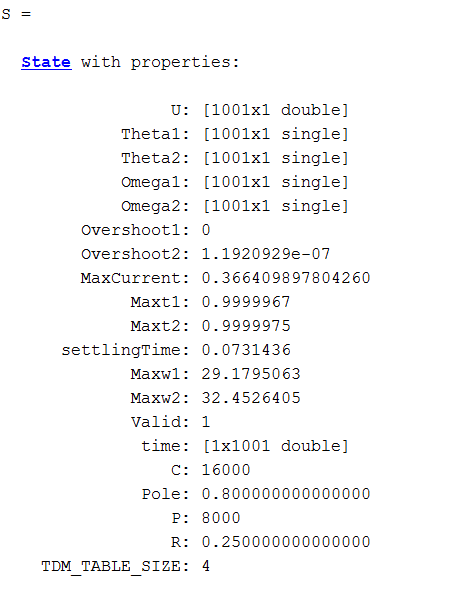
\includegraphics[width=0.5\linewidth]{img/S}
		\caption{State object of the system and its properties. This shows the values for the best solution found. The values will be explained throughout the report}
		\label{fig:S}
	\end{center}
\end{figure}

\begin{figure}[h!]
	\begin{center}
		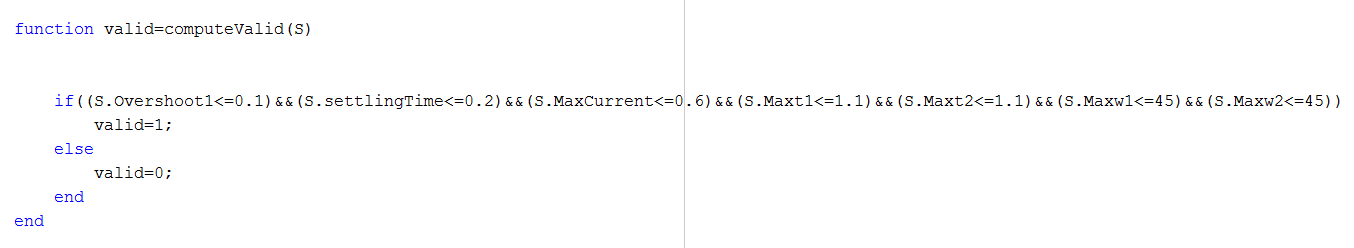
\includegraphics[width=1.1\linewidth]{img/valid}
		\caption{Validating design requirements condition on State Object.}
		\label{fig:valid}
	\end{center}
\end{figure}



\begin{enumerate}
	\item First tests made were rather basic and were used to determine the acuteness of poles on the system. A Matlab script was made to keep P=C,from 5000 up to 16000 clock cycles, and alternating the poles from 0.6 up to 0.9 with 0.1 as increment(keeping all poles at the same value). Along each test, settling time and validity of design constraints was included as output. Thus the valid parameter would render 0 or 1 depending on if all design constraints are met or not.
	
	To clarify all combinations of the following were tested, 40 in total:
	\begin{description}
		\item[P=C=] [5000:1000:16000]
		\item[Poles=] [0.6:0.1:0.9]$\cdot$[1 1 1 1 1]
		\item[TDM Table Size] = 4
	\end{description}
	When poles were at 0.6 and 0.7 there were very few valid options so these were excluded.
	
	\item Then ruling out poles at 0.6 and 0.7 and sticking to 0.8 and 0.8 where that gave more promising results. Then adding a fraction relation between C and P as shown here:
		\begin{description}
			\item[P=$\dfrac{C}{frac}$] where frac = [1:0.1:2]
			\item[Poles=] [0.8:0.1:0.9]$\cdot$[1 1 1 1 1]
			\item[TDM Table Size] = 4
		\end{description}
	This yielded around \textbf{200 options} both valid and invalid counted.
	\item Now filter out only valid results, which meet the design constraints set such as settling time and current limitations (and a few more). This is yielded to \textbf{102 valid options}.
	\item Next calculate the Quality of Control and R for each of the valid option which then allows for calculating a cost function(QoC/R) for each of the 102 options.
	\item Now all of the options chosen at this point are valid but the cost function will allow us to determine the most promising ones even though this done for a fixed TDM table size. Out of these 102, the top candidates were chosen and are investigated further, these are shown in Table \ref{tab:list}. The higher the ranking, the better the options is considered to be. Where options with pole at 0.8 are a bit more unstable when settling time is up, the best options representing poles at 0.9 was also chosen even though it considerable worse ranking it proofs to be more stable.
	
	\begin{table}[htbp]
		\centering
		\caption{Options for platform parameters derived from numerous investigations and scripts. Higher ranking indicates overall better performance. Poles are chosen identical for all five of them. TDM table size it constant at 4.}
		\begin{tabular}{lllccccc}
			\toprule
			Rank & C& P & Poles &Valid &OoC & R & $\dfrac{QoC}{R}$ [Cost Function] \\ 
		\midrule
		\textbf{102} & \textbf{16000} & \textbf{8000} & \textbf{0.8} & \textbf{{1}} & \textbf{\textcolor{blue}{18.34}} & \textbf{0.2500} &\textbf{ 73.34} \\ 
		101 & 15000 & 7895 & 0.8 & 1 & 18.39 & 0.2586 & 71.11 \\ 
		100 & 16000 & 8421 & 0.8 & 1 & 18.34 & 0.2586 & 70.90 \\ 
		99 & 8000 & 4000 & 0.9 & 1 & 17.51 & 0.2500 & 70.05 \\ 
		\textbf{{98}} & \textbf{{7000}} & \textbf{{3500}} & \textbf{{0.9}} & \textbf{ {1}} &\textbf{ \textcolor{blue}{17.51}} & \textbf{{0.2500}} & \textbf{{70.05}} \\ 
		97 & 15000 & 8333 & 0.8 & 1 & 18.39 & 0.2679 & 68.65 \\ 
		96 & 10000 & 5000 & 0.9 & 1 & 17.12 & 0.2500 & 68.49 \\
		\midrule 
		\textbf{21} & \textbf{16000}& \textbf{8000}& \textbf{0.9}&\textbf{{1}}&\textbf{\textcolor{blue}{8.10}}&\textbf{{0.2500}}&\textbf{{32.38}}\\
		
	\midrule
	\end{tabular}
	\label{tab:list}
\end{table}



	\item Now when some good values for P, C and the poles had been chosen it is a good time to look at the TDM table sizes. This is also covered in more detail in Section \ref{sec:codesign}.


\end{enumerate}

\subsubsection{Sensor to actuator delay}
\label{sec:stad}

The sensor to actuator delay is the time in the control system it takes from sensor input until computed and actuator actuates. This time is then highly related to P, C, TDM table size, Global clock frequency and sampling period. The exact delay can be precisely calculated per Equation \ref{eq:delay}. And number are put in according to one of the options determined for the controls system from Table \ref{tab:list}.

\begin{equation}
	\text{Exact Delay}=(C+P)\cdot NUMTASKS  = (16000+8000)\cdot 3  = 72000 \text{ clock cycles}
	\label{eq:delay}
\end{equation}
\begin{equation}
	\text{Rounded Delay}= \text{ceil}\left(\dfrac{\text{Exact Delay}}{\text{Plant Sampling Period}}\right) \cdot \text{Plant Sampling Period} = 80000 \text{ clock cycles}
\label{eq:rounddelay}
\end{equation}

\begin{equation}
\text{Delay}=\text{Rounded Delay} - \text{Exact Delay}= 8000 \text{ clock cycles}
\label{eq:delayall}
\end{equation}

Then when substituting 8000 for the delay in sconfig.c the output file gave error regarding timing that the delay might be to long. The reason might be because the delay landed just on the other side of the next task so reducing the delay to 7000 clock cycles did the trick and the results matched the Simulink results.

%\subsection{Implementation of Design steps in Matlab}
%\color{red}
%Show Matlab code for designing and explain matlab approach. Would be great if you, Sai, could just put some code snippets from matlab. Like some part of the looptrhough code where the valid parameters is gotten for example or your cool objects ;).
%\color{black}

%\begin{lstlisting}[language=matlab,caption={Matlab code showing the loopthrough function }]
%Matlab code
%\end{lstlisting}



\section{Co-Design Aspects}
\label{sec:codesign}
\color{red}
Co-design	aspects,	e.g.,	necesity for	re-design.	Your	design	decision	and	justification
\color{black}
While above sections describe formulating initial design that satisfy design constraints, this section deals with obtaining an optimal one. For this purpose an automated script is built to search through the search space for obtaining an optimal solution. Following observations are made from the experiments.

\begin{enumerate}
	\item TDM frame size is inversely proportional to QOC. This is because less are the number of slots allocated to application more is the delay between successive samplings. This makes the system to respond slowly i.e higher settling time and lesser control. On the contrary when more slots are allocated to the application the delay between successive samplings is reduced and hence better control. But again when the resource utilization is high, i.e when almost all the slots are allocated to the application, it makes the system to respond rapidly and when adequate measures are not taken might result in an unstable system.
	
	\item A similar argument can be made for an increment in the slot size in the frame. Higher the slot size more is the frame size, higher the sampling period and lesser is the control. However in this case the resource utilization depends on the ratio of slot sizes P and C. Therefore lesser the slot size  doesn't necessarily imply a better QOC vs R graph.
	
	\item Placement of poles control the damping factor of the system effecting the rate at which the system responds. Closer the poles more rapid is the response. Poles very close might result in large overshoots driving the system unstable. This calls for a optimal pole selection, a trade-off between QOC and stability.
\end{enumerate}

\begin{figure}[h]
	\begin{center}
		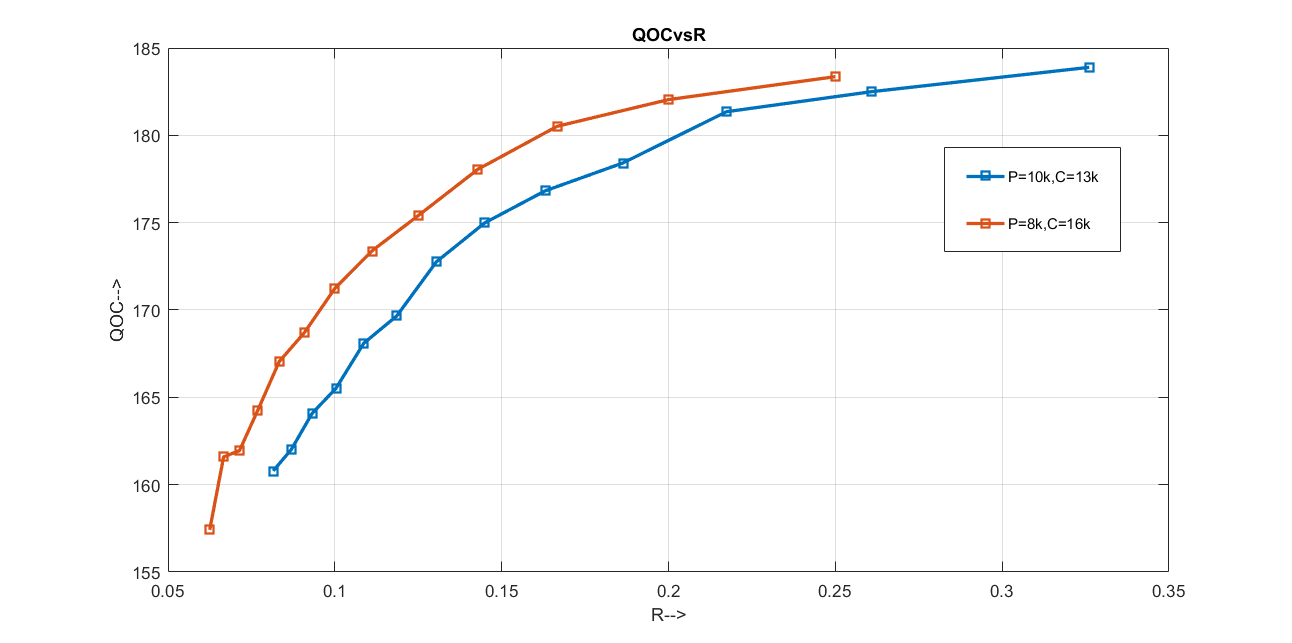
\includegraphics[width=\linewidth]{img/qoc2}
		\caption{QOC vs R for different C and P. Here all poles are at 0.8 for both plots. Showing first two options in Table \ref{tab:list}}
		\label{fig:qoc2}
	\end{center}
\end{figure}
\section{Results}


\color{red}
Results:	control	input,	system	states,	comment	on	the	requirements,	and	comparisons	
between	CompSOC and	MATLAB	outcomes
\color{black}

%Results:	control	input,	system	states,	comment	on	the	requirements,	and	comparisons	
%between	CompSOC and	MATLAB	outcomes

\begin{figure}[h]
	\begin{center}
		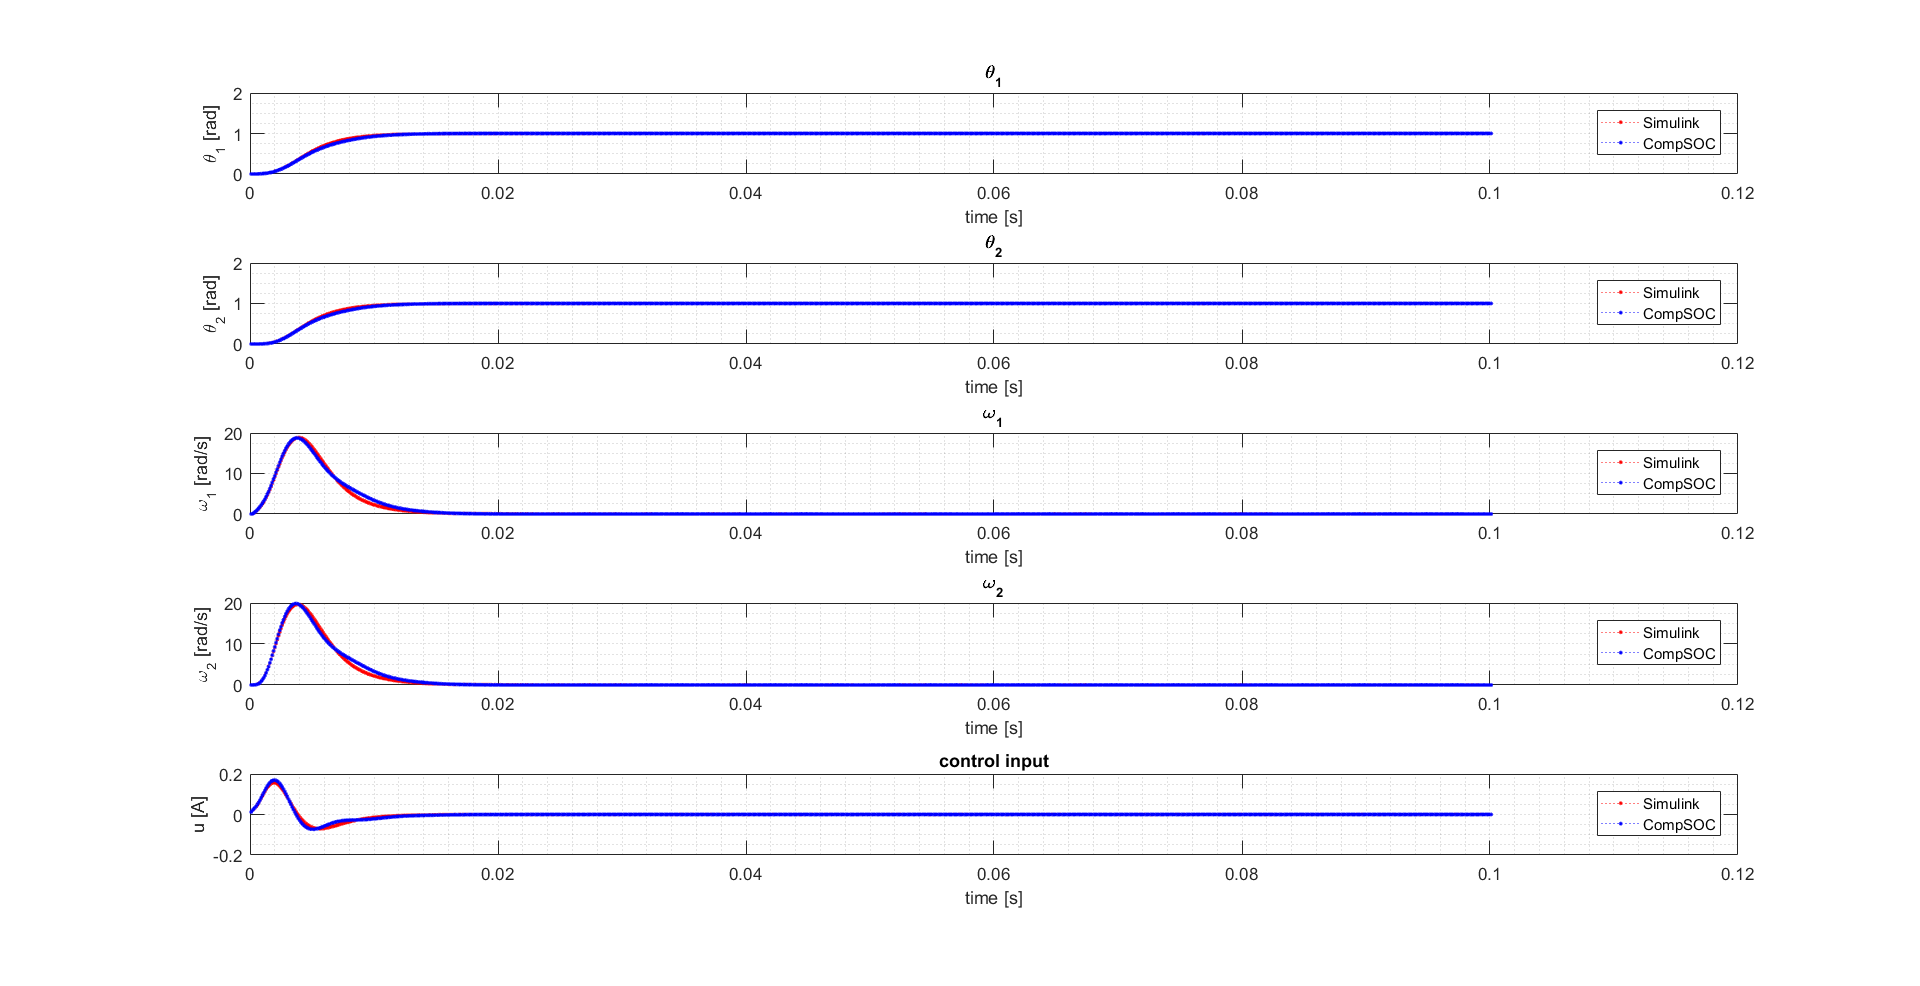
\includegraphics[width=\linewidth]{img/finalresult}
		\caption{Results comparison from Simulink and CompSOC.}
		\label{fig:finalresult}
	\end{center}
\end{figure}

\section{Conclusion}
%• Conclusions

Also see:
\begin{enumerate}
	\item Modified	CompSOC configuration	file	(sconfig.c)
	\item System	states	and	control	input	traces	from	the	CompSOC platform	(states.txt,	
	input.txt)
	\item Makefile used	to	specify	the	USER_TIMEOUT	(makefile)
	\item MATLAB	control	design	script	(stud_control_design_a1.m)
\end{enumerate}



\printbibliography

\end{document}

